\section{Veto Efficiency Measurement with a Collimated $^{137}$Cs Source}
\label{secVetoEfficiencyMeasurement}


From the Monte Carlo simulations of the light collection for the S1 signal (Section~\ref{secLCEs1}) it is known that the response in the liquid xenon veto is very non-uniform. The predicted light yield in the side and top veto is shown in Fig.~\ref{figLCEvetoMC}. It has been calculated by scaling the simulated LCE to the volume-averaged light yield of 3.18~pe/keV in the liquid xenon target, which has been measured at 662~keV. 

The LCE in the veto volume is affected by various components, i.e. cables, which are difficult to properly take into account in the modeling of photon collection. In addition, light yield is quenched by the electric field present in the veto. 
In order to correctly determine the energy threshold in the different regions of the veto volume, a detailed measurement of the light yield in the veto has been performed with a collimated $^{137}$Cs source. 
The lead collimator used for the measurements had the dimensions 28$\times$50$\times$32~mm$^{3}$, and a collimator hole with a radius of 3.7~mm and a length of 16~mm. The $^{137}$Cs source had an activity of 68.9~kBq at the time when the measurements were performed. 
In the side veto, measurements at 60 points have been performed, marked and labeled in Fig.~\ref{figLCEvetoMC_1}. To ensure that the collimator is set correctly, the positioning has been done with millimeter paper fixed on the cryostat, shown in Fig.~\ref{figVetoMapping_1}. The measurement points on the top of the cryostat are indicated in Fig.~\ref{figVetoMapping_2}.

\begin{figure}[!h]
\centering
\subfigure[side veto]{
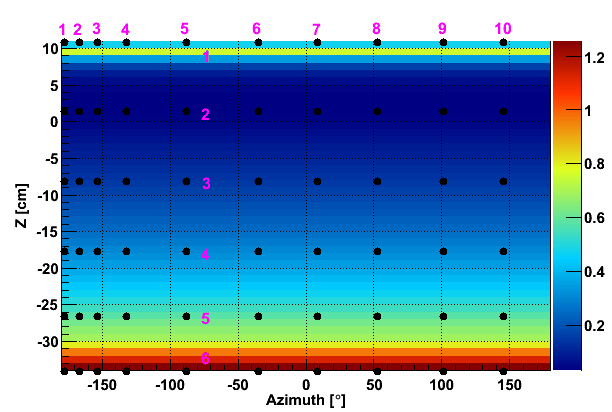
\includegraphics[height=0.35\linewidth]{plots/VetoMeasurement/mapLY_ZsideVeto_withMarkers.png}
\label{figLCEvetoMC_1}}
\subfigure[top veto]{
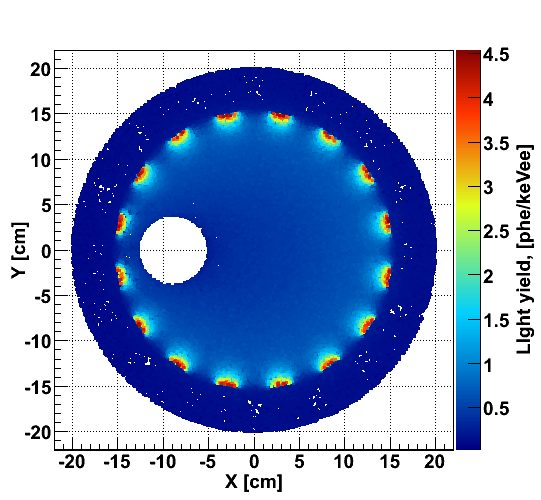
\includegraphics[height=0.36\linewidth]{plots/VetoMeasurement/map_topVeto_withMarkers.png}
\label{figLCEvetoMC_2}}
\caption[Simulated light yield at zero field in the side veto and top veto volumes]{Simulated light yield at zero field in the side veto (a) and top veto (b) volumes. The black markers in figure (a) indicate the measurement points. The empty spot in figure (b) corresponds to the position of the pipe which guides the PMT cables.}
\label{figLCEvetoMC}
\end{figure}

\begin{figure}[!h]
\centering
\subfigure[side]{
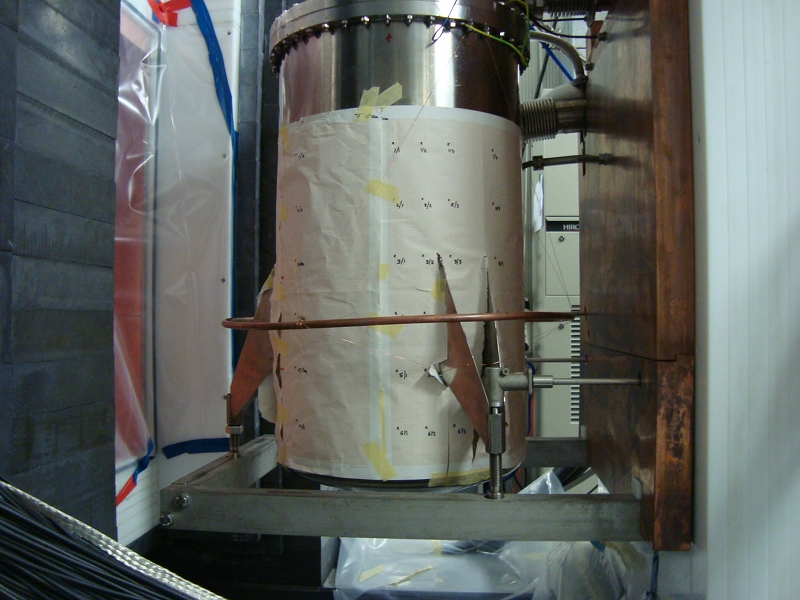
\includegraphics[height=0.3\linewidth]{plots/VetoMeasurement/SideVetoMapping.png}
\label{figVetoMapping_1}}
\subfigure[top]{
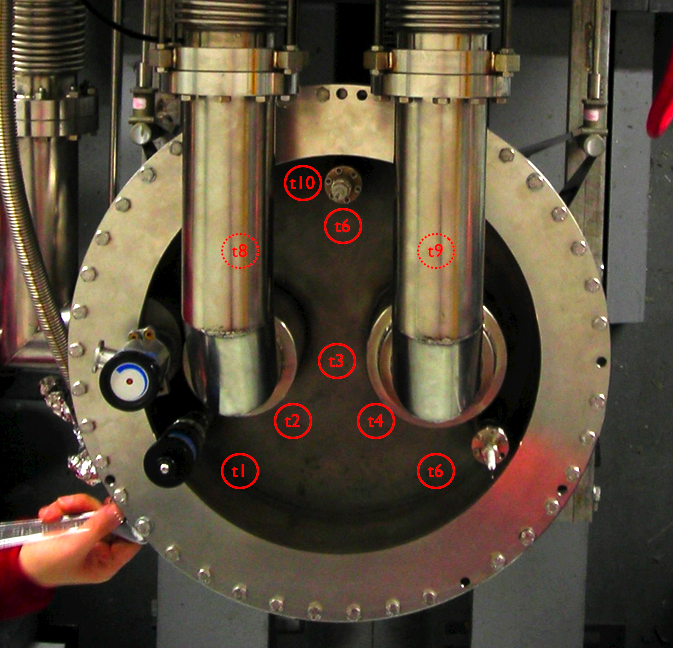
\includegraphics[height=0.3\linewidth]{plots/VetoMeasurement/TopVetoMapping.png}
\label{figVetoMapping_2}}
\caption[Mapping of the measurement points in the side veto marked on millimeter paper, and measured points above top veto volume]{Mapping of the measurement points in the side veto marked on millimeter paper (a), and measured points above top veto volume (b).}
\label{figVetoMapping}
\end{figure}

\begin{table}[!b]
\centering
\caption[Vertical positions for measurements of the energy threshold in the veto volume with a collimated $^{137}$Cs source]{Vertical positions for measurements of the energy threshold in the veto volume with a collimated $^{137}$Cs source. The systematic uncertainty is $\pm$5~mm.}
\label{tabVetoCoordinatesVertical}
%\vspace{0.2cm}
\begin{tabular}{>{\footnotesize}l|>{\footnotesize}c|>{\footnotesize}c|>{\footnotesize}c|>{\footnotesize}c|>{\footnotesize}c|>{\footnotesize}c}
%\footnotesize
\hline
\footnotesize{Position number}			& 1 				& 2				& 3				& 4 	 			& 5				& 6 \\
\hline
Coordinate [cm] & & & & & & \\
\ \ relative to the top flange	      		& 28.5$\pm$0.5	& 37.0$\pm$0.5 	& 46.5$\pm$0.5	& 56.0$\pm$0.5 	& 65.0$\pm$0.5	& 72.5$\pm$0.5 \\
\ \ relative to the liquid surface		& 10.9$\pm$0.5	& 1.4$\pm$0.5 		& -8.2$\pm$0.5		& -17.7$\pm$0.5 	& -26.7$\pm$0.5	& -34.2$\pm$0.5 \\
\hline
\end{tabular}
\end{table}

The coordinates of the 6 vertical positions are listed in Table~\ref{tabVetoCoordinatesVertical}, measured relative to the top of the cryostat flange, and relative to the liquid-gas interface. The polar coordinates for the 10 azimuthal positions are listed in Table~\ref{tabVetoCoordinatesAzimuthal}, where angle $\Theta$ has been defined in the range [$-\pi$,$\pi$], and $\Theta$ = 0 has been set at $Y$ = 0. The systematic uncertainty of the collimator adjustment for the vertical positions is $\pm$5~mm, and $\pm$1.3$^{\circ}$ for the azimuthal positions.

\begin{table}[!h]
\centering
\caption[Azimuthal positions for side veto mapping with a collimated $^{137}$Cs source]{Azimuthal positions for side veto mapping with a collimated $^{137}$Cs source. The polar angle is defined in the interval [-$\pi$,$\pi$]. The systematic uncertainty on the measured angle is 1.3$^{\circ}$. }
\label{tabVetoCoordinatesAzimuthal}
%\vspace{0.2cm}
\begin{tabular}{>{\footnotesize}l|>{\footnotesize}c|>{\footnotesize}c|>{\footnotesize}c|>{\footnotesize}c|>{\footnotesize}c|>{\footnotesize}c|>{\footnotesize}c|>{\footnotesize}c|>{\footnotesize}c|>{\footnotesize}c}
%\footnotesize
\hline
\footnotesize{Position number}		& 1 		& 2		& 3		& 4 	 	& 5		& 6		& 7		& 8		& 9		& 10 \\
\hline
Polar angle [$^{\circ}$]	      	& -177.5	& -166.8 	& -153.7	& -131.7 	& -87.8	& -35.5 	& 8.8		& 52.7	& 101.0	& 144.9 \\
\hline
\end{tabular}
\end{table}

\begin{figure}[!t]
\centering
\subfigure[]{
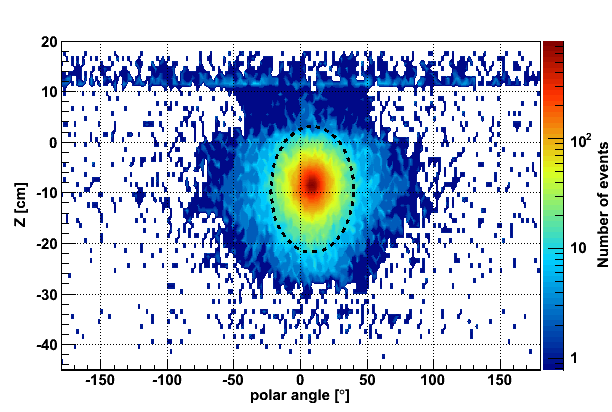
\includegraphics[width=0.475\linewidth]{plots/VetoMeasurement/Cs137inCollimator_AZ_MC_pos37_with3sigma.png}
\label{figCollimatorMC_1}}
\subfigure[]{
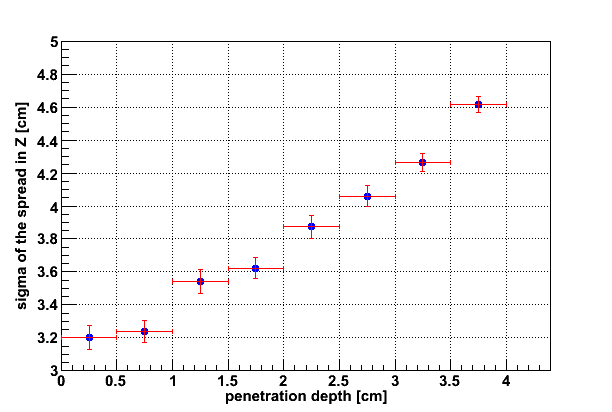
\includegraphics[width=0.475\linewidth]{plots/VetoMeasurement/Cs137inCollimator_sigmaZvsDepth.png}
\label{figCollimatorMC_2}}
\caption[Monte Carlo simulation of the collimated $^{137}$Cs source, and the spread of the collimated beam as a function of the penetration depth in liquid xenon]{(a) - Monte Carlo simulation of the collimated $^{137}$Cs source in position 3/7 (defined in Tables~\ref{tabVetoCoordinatesVertical} and \ref{tabVetoCoordinatesAzimuthal}). Dashed ellipse shows the 3$\sigma$ spread of the $\gamma$-beam. (b) - the spread of the collimated beam ($\sigma$) as a function of the penetration depth in liquid xenon.}
\label{figCollimatorMC}
\end{figure}

\begin{figure}[!b]
\begin{center}
%\begin{tabular}{cc}
%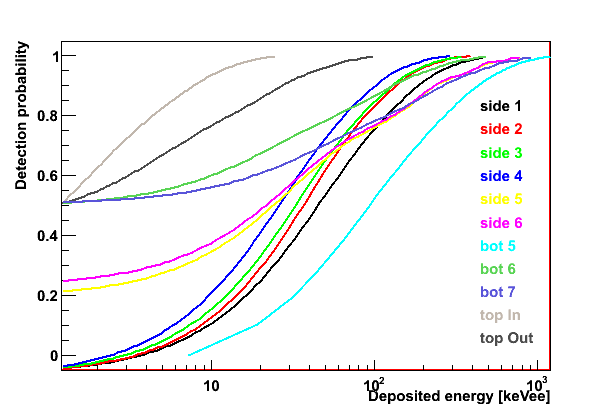
\includegraphics[width=0.475\linewidth]{plots/VetoMeasurement/polinomials.png}
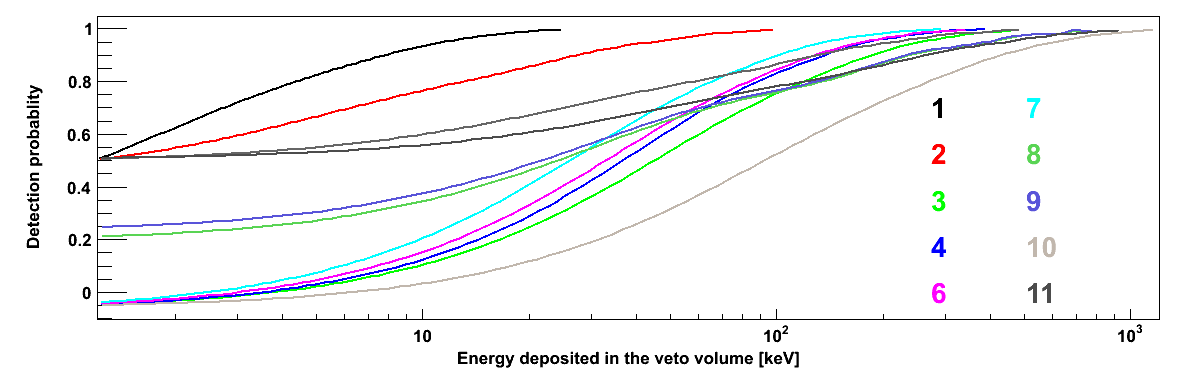
\includegraphics[width=1.0\linewidth]{plots/VetoMeasurement/VetoRegions.png}
%\end{tabular}
\caption[Detection efficiency in the veto as a function of the deposited energy for different parts of the veto volume]{Detection efficiency in the veto as a function of the deposited energy for different regions of the veto volume. The curves stop at the energies where detection efficiency is unity.  The regions are defined in Fig.~\ref{figAZveto_1}.}
\label{figPolynomials}
\end{center}
\end{figure}

A Monte Carlo simulation has been performed with GEANT4 in order to determine the position dependence of the energy deposition from the collimated $^{137}$Cs source in the side veto volume. Even though the source was collimated, it still probes a rather large region~(Fig.~\ref{figCollimatorMC_1}), which has an advantage that not too many positions have to be measured to avoid not calibrated regions. The collimation is characterized by fitting the events distribution with a two-dimensional gaussian function, which gives $\sigma$ of 4.2~cm and 10.4$^{\circ}$ for the vertical and azimuthal coordinates, respectively. The mean free path of 662~keV $\gamma$-rays in liquid xenon is $\sim$4cm, similar to the thickness of the side veto layer. Therefore, the spread of events with full $\gamma$-absorption increases with the penetration depth (Fig.~\ref{figCollimatorMC_2}). In the regions close to the PMTs where the LCE is subject to large variations, this effect leads to a rather wide energy spectrum with a badly defined full absorption peak, and results in impossibility to resolve the fine structures in LCE. Hence, for some regions only the integral effect has been measured, and the energy thresholds have been determined as conservative upper limits, using the full spectrum with the Compton continuum.

All measurements have been combined into 11 functions, which describe the detection probability as a function of the deposited energy. They are shown in Fig.~\ref{figPolynomials}, and the corresponding regions are indicated on the simulated S1 LCE map in Fig.~\ref{figAZveto_1}. The 90\% detection thresholds have been determined to be between 180~keV and 235~keV in the side veto, 130~keV below the bottom PMT array, 10-30~keV above the target volume, and about 450~keV in the regions behind the PMTs, resulting in a volume averaged energy threshold of 100~keV.

The measured energy threshold in the veto volume has been implemented into Monte Carlo simulations using the functions shown in Fig.~\ref{figPolynomials}. The event distribution in the veto volume without and with the veto coincidence cut is shown for the predicted background (for details see Chapter~\ref{chERbackground}) in Fig.~\ref{figAZveto_2} and Fig.~\ref{figAZveto_3}, respectively. The events remaining after the veto coincidence cut are below the energy threshold, and indicate veto regions with relatively low detection efficiency.

\begin{figure}[!h]
\centering
\subfigure[LCE]{
%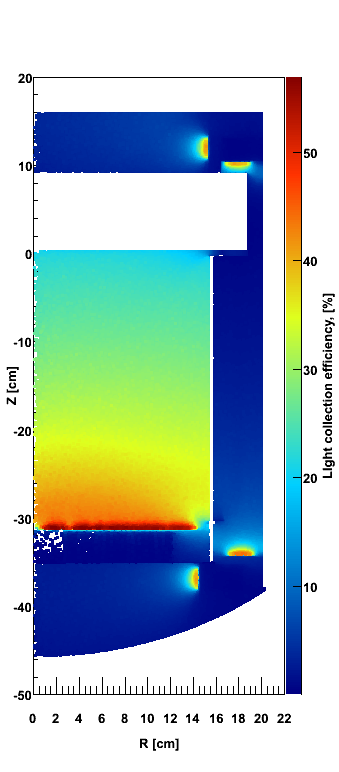
\includegraphics[height=0.5\linewidth]{plots/VetoMeasurement/RZhits_colors_nogrid.png}
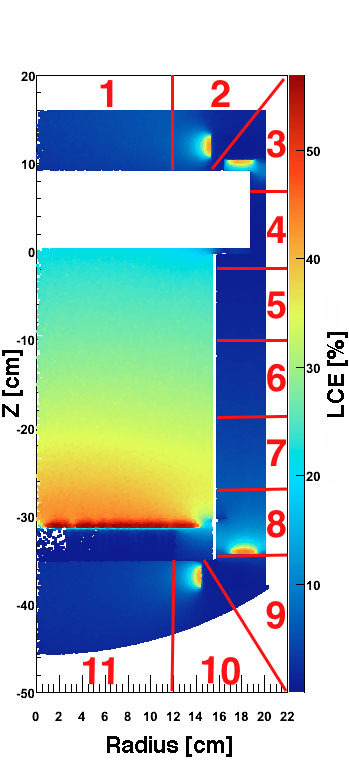
\includegraphics[height=0.5\linewidth]{plots/VetoMeasurement/RZregions.png}
\label{figAZveto_1}}
\subfigure[BG, no veto cut]{
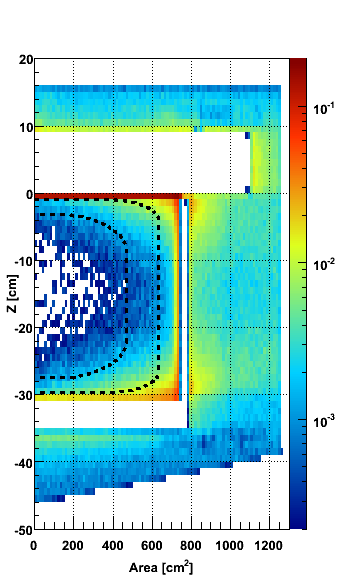
\includegraphics[height=0.5\linewidth]{plots/VetoMeasurement/AZ_targetVeto_passive.png}
\label{figAZveto_2}}
\subfigure[BG, with veto cut]{
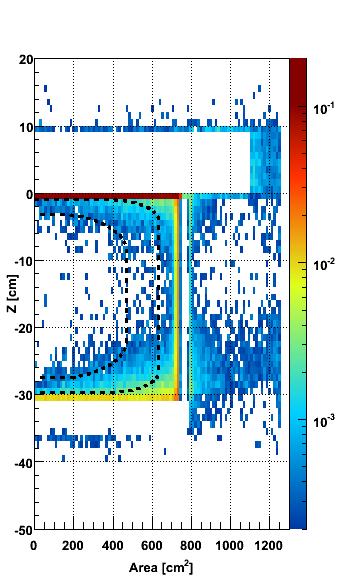
\includegraphics[height=0.5\linewidth]{plots/VetoMeasurement/AZ_targetVeto_active.png}
\label{figAZveto_3}}
\caption[Veto regions with different energy threshold on a simulated S1 LCE map, and simulated spatial distribution of events without and with a veto coincidence cut]{(a) - simulated S1 light collection efficiency indicating the veto regions with different energy thresholds. (b) and (c) - spatial distribution of events in the simulated electromagnetic background, without and with the veto coincidence cut. The events left in figure (c) are below energy threshold in the veto.}
\label{figAZveto}
\end{figure}


%\begin{figure}[!h]
%\centering
%\subfigure[]{
%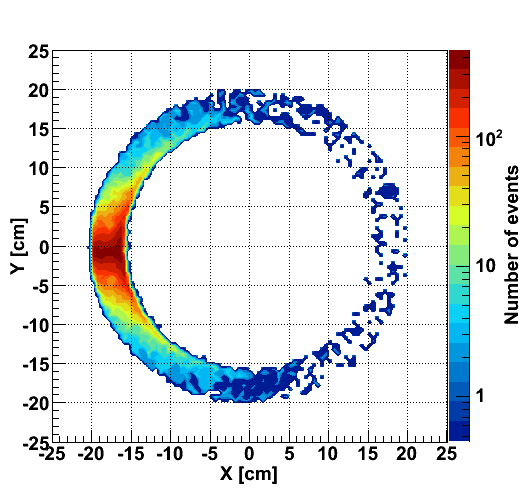
\includegraphics[width=0.375\linewidth]{plots/VetoMeasurement/Cs137inCollimator_XY_MC_pos31_colP.png}
%\label{figCollimatorMC_1}}
%\subfigure[]{
%\label{figCollimatorMC_2}}
%\caption{Monte Carlo simulation of the collimated $^{137}$Cs source in position 3/1. Events distribution in XY plane. MC simulation of the position 3/7. Dashed ellipse shows the solid angle of the events distribution, based on 3$\sigma$ values of the spread.}
%\label{figCollimatorMC}
%\end{figure}


%\begin{figure}[!h]
%\begin{center}
%\begin{tabular}{cc}
%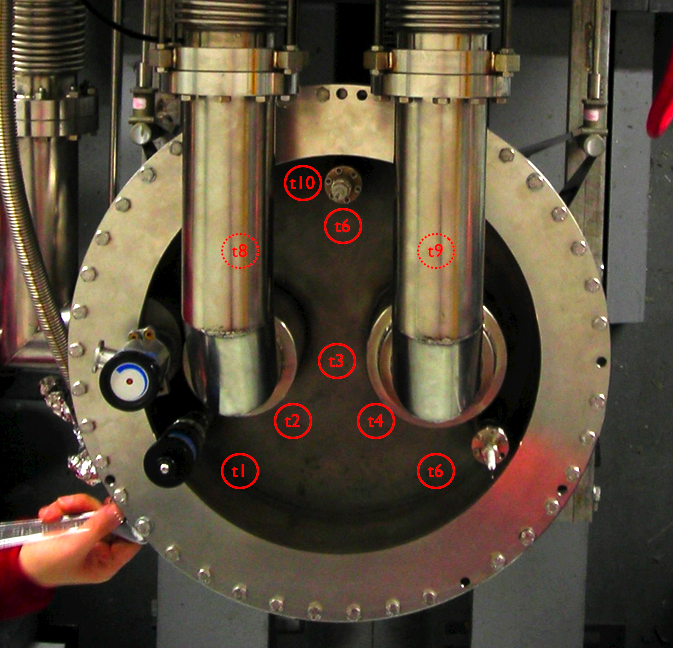
\includegraphics[height=0.3\linewidth]{plots/VetoMeasurement/TopVetoMapping.png}
%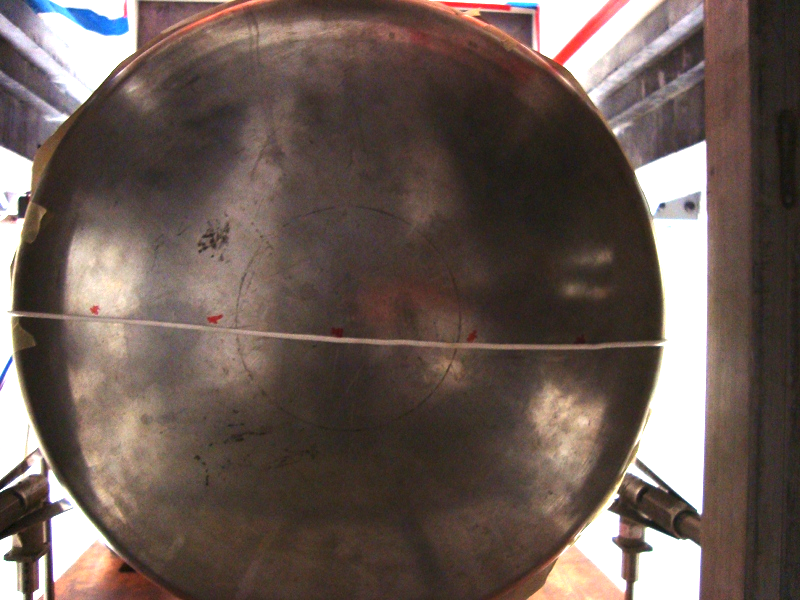
\includegraphics[height=0.3\linewidth]{plots/VetoMeasurement/BottomVetoMapping.png}
%\end{tabular}
%\caption{Measurements of the top and bottom veto.}
%\label{figVetoTopBottom}
%\end{center}
%\end{figure}


%\begin{figure}[!h]
%\begin{center}
%\begin{tabular}{cc}
%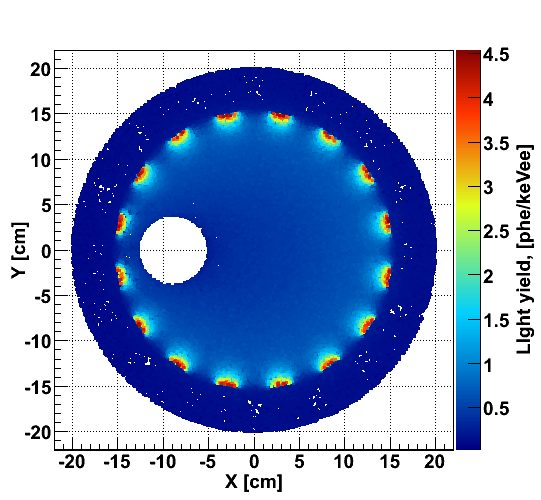
\includegraphics[height=0.3\linewidth]{plots/VetoMeasurement/map_topVeto_withMarkers.png}
%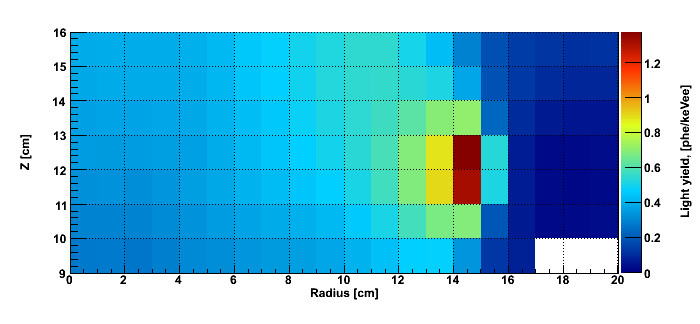
\includegraphics[height=0.3\linewidth]{plots/VetoMeasurement/map_topVeto.png}
%\end{tabular}
%\caption{Simulated light collection in the top veto.}
%\label{figVetoTopMC}
%\end{center}
%\end{figure}


%\begin{figure}[!h]
%\centering
%\subfigure[]{
%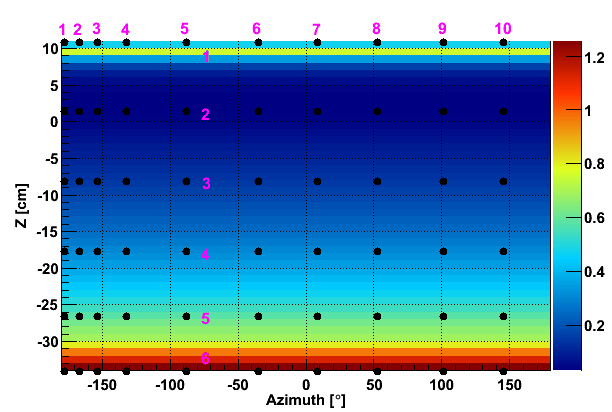
\includegraphics[height=0.35\linewidth]{plots/VetoMeasurement/mapLY_ZsideVeto_withMarkers.png}
%\label{figSideVetoPos_1}}
%\subfigure[]{
%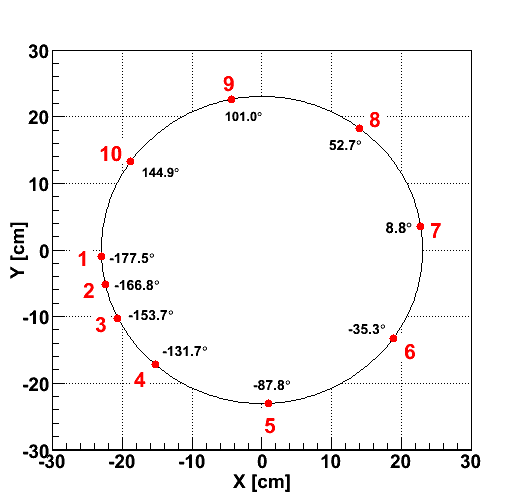
\includegraphics[height=0.35\linewidth]{plots/VetoMeasurement/CircleWithAzimuthalPositions.png}
%\label{figSideVetoPos_2}}
%\caption{Vertical and azimuthal positions.}
%\label{figSideVetoPos}
%\end{figure}


